% This is text associated with the open textbook "Open Electromagnetics"
% See immediately below for author, date
% This work is licensed under the Creative Commons Attribution-ShareAlike 4.0 International License. (CC BY-SA 4.0) 
% To view a copy of the license, visit http://creativecommons.org/licenses/by-sa/4.0/

%ORB TITLE Microstrip Line Redux
%ORB AUTHOR 0        # S.W. Ellingson, Virginia Tech (ellingson@vt.edu)
%ORB DATE 20191202   # yyyymmdd
%ORB ABSTRACT  

\label{m0186_Microstrip_Line_Redux} % <-- Must match name of this file and module directory name.  Don't mess with this!
\index{transmission line!microstrip|see{microstrip}}
\index{microstrip|(}

A microstrip transmission line consists of a narrow metallic trace separated from a metallic ground plane by a slab of dielectric material, as shown in Figure~\ref{m0186_fMicrostripCrossSection}. 
This is a natural way to implement a transmission line on a printed circuit board,
\index{printed circuit board (PCB)}
and so accounts for an important and expansive range of applications.
The reader should be aware that microstrip is distinct from \emph{stripline},
\index{stripline}
\index{transmission line!stripline}
which is a distinct type of transmission line; see ``Additional Reading'' at the end of this section for disambiguation of these terms.
%
\begin{figure}[b!] % <--- "[b]" for first figure in section *only*; delete for 2nd and subsequent figures
\begin{center}
\pdftooltip{{  % note double braces
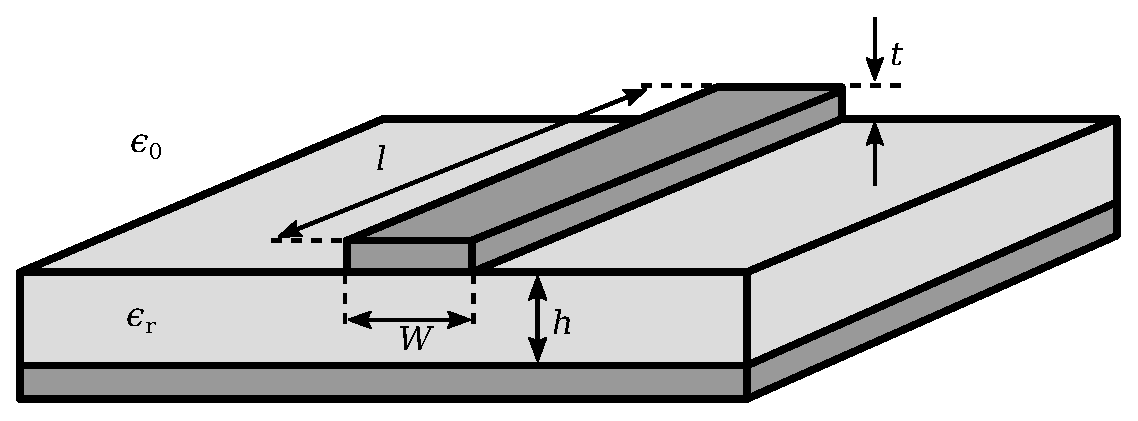
\includegraphics[width=\columnwidth]{modules/m0186_fMicrostripCrossSection.eps}
% https://commons.wikimedia.org/wiki/File:Microstrip_scheme.svg
}}{A diagram of a microstrip transmission line. Certain dimensions are labeled: Length of the metal trace (l), width of the metal trace (W), thickness of the metal trace (t), and height of the dielectric slab (h). Epsilon sub r is labeled on the dielectric and epsilon sub 0 is labeled on the space next to the microstrip transmission line.}
\end{center} 
\centerline{\scriptsize 
\copyright~\hyperref[m0186_fMicrostripCrossSection_Credit]{7head7metal7}  
\href{https://creativecommons.org/licenses/by-sa/3.0/}{CC BY~SA 3.0} 
(modified)
} 
\caption{
\label{m0186_fMicrostripCrossSection}
Microstrip transmission line structure and design parameters.
}
\end{figure}

A microstrip line is single-ended\footnote{The reference in ``Additional Reading'' at the end of this section may be helpful if you are not familiar with this concept.} 
\index{transmission line!single-ended}
in the sense that the conductor geometry is asymmetric and the one conductor -- namely, the ground plane -- also normally serves as ground for the source and load.

The spacer material is typically a low-loss dielectric 
\index{dielectric (material)}
material having permeability approximately equal to that of free space ($\mu \approx \mu_0$) and relative permittivity $\epsilon_r$ in the range of 2 to about 10 or so.

The structure of a microstrip line is similar to that of a parallel plate waveguide (Section~\ref{m0220_Parallel_Plate_Waveguide_TM0_Mode}), with the obvious difference that one of the ``plates'' has finite length in the direction perpendicular to the direction of propagation.
Despite this difference, the parallel plate waveguide provides some useful insight into the operation of the microstrip line.  
Microstrip line is nearly always operated below the cutoff frequency 
\index{cutoff frequency}
of all but the TM$_0$ mode, whose cutoff frequency is zero.
This guarantees that only the TM$_0$ mode can propagate.
The TM$_0$ mode has the form of a uniform plane wave, as shown in Figure~\ref{m0186_fMicrostripFieldStructure}. 
The electric field is oriented in the direction perpendicular to the plates, and magnetic field is oriented in the direction parallel to the plates.
The direction of propagation ${\bf E}\times{\bf H}$ for the TM$_0$ mode always points in the same direction; namely, along the axis of the transmission line. Therefore, microstrip lines nominally exhibit transverse electromagnetic (TEM) 
\index{transmission line!transverse electromagnetic (TEM)}
field structure.
%
\begin{figure}
\begin{center}
\pdftooltip{{  % note double braces
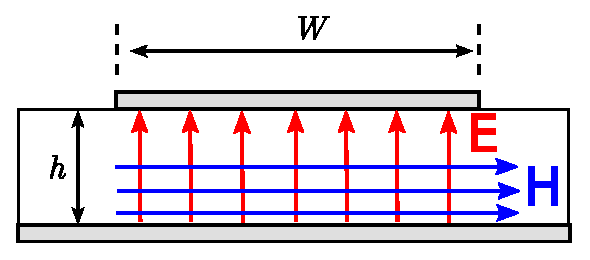
\includegraphics[width=2.5in]{modules/m0186_fMicrostripFieldStructure.eps}
}}{A cross-sectional view of the microstrip transition line. The electric field, "E", is represented by a row of red parallel arrows pointing vertically from the ground plane to the metallic trace.The magnetic field, "B", is represented by parallel blue arrows perpendicular to the electric field arrows, pointing to the right.}
\end{center} 
\caption{\label{m0186_fMicrostripFieldStructure}{\it Approximate} structure of the electric and magnetic fields within microstrip line, assuming TM$_0$ operation. The fields \emph{outside} the line are possibly significant, complicated, and not shown.  In this case, the wave is propagating away from the viewer.}
\end{figure}
  
The limited width $W$ of the trace results in a ``fringing field'' -- i.e., significant deviations from TM$_0$ field structure in the dielectric beyond the edges of the trace and above the trace.
The fringing fields may play a significant role in determining the characteristic impedance 
\index{characteristic impedance}
$Z_0$. 
Since $Z_0$ is an important parameter in the analysis and design of systems using transmission lines, we are motivated to not only determine $Z_0$ for the microstrip line, but also to understand how variation in $W$ affects $Z_0$.
Let us address this issue by considering the following three special cases, in order: 
\begin{itemize}
\item $W \gg h$, which we shall refer to as the ``wide'' case.
\item $W \ll h$, which we shall refer to as the ``narrow'' case.
\item $W \sim h$; i.e., the intermediate case in which $h$ and $W$ equal to within an order of magnitude or so.
\end{itemize}

{\bf Wide case.}  If $W \gg h$, most of the energy associated with propagating waves lies directly underneath the trace, and Figure~\ref{m0186_fMicrostripFieldStructure} provides a relatively accurate impression of the fields in this region.
The characteristic impedance $Z_0$ may be determined using the ``lumped element'' transmission line model 
\index{transmission line!lumped-element model}
using the following expression:
%
\begin{equation}
Z_0 = \sqrt{\frac{R'+j\omega L'}{G'+j\omega C'}}
\end{equation}
%
where $R'$, $G'$, $C'$, and $L'$ are the resistance, conductance, capacitance, and inductance per unit length, respectively.
For the present analysis, nothing is lost by assuming loss is negligible; therefore, let us assume $R' \ll \omega L'$ and $G' \ll \omega G'$, yielding
%
\begin{equation}
Z_0 \approx \sqrt{\frac{L'}{C'}}
\end{equation}
%
Thus the problem is reduced to determining capacitance and inductance of the transmission line.

Wide microstrip line resembles a parallel-plate capacitor whose plate spacing $d$ is very small compared to the plate area $A$.
In this case, fringing fields may be considered negligible and one finds that the capacitance $C$ is given by
%
\begin{equation}
C \approx \frac{\epsilon A}{d} ~~~ \mbox{(parallel plate capacitor)}
\end{equation}
%
In terms of wide microstrip line, $A=Wl$ where $l$ is length, and $d=h$.  Therefore:
%
\begin{equation}
C' \triangleq \frac{C}{l} \approx \frac{\epsilon W}{h} ~~~ (W \gg h)
\end{equation}

To determine $L'$, consider the view of the microstrip line shown in Figure~\ref{m0186_fMicrostripLp}.
%
\begin{figure}% <--- "[b]" for first figure in section *only*; delete for 2nd and subsequent figures
\begin{center}
\pdftooltip{{  % note double braces
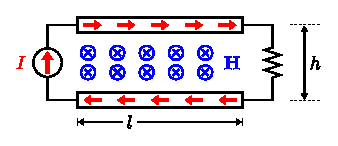
\includegraphics[width=2.5in]{modules/m0186_MicrostripLp.eps}
% https://commons.wikimedia.org/wiki/File:View_from_the_side_of_a_microstrip_line.svg
}}{A closed loop circuit has a current source on the left vertical branch and the right vertical branch has a resistive load. Each horizontal line has a strip. The steady current flows continuously from current source through upper strip, through resistive load and then through lower strip. Magnetic field intensity capital H is directed into the page.}
\end{center} 
\centerline{\scriptsize 
\copyright~\hyperref[m0186_fMicrostripLp_Credit]{C.\ Wang}  
\href{https://creativecommons.org/licenses/by-sa/4.0/}{CC BY~SA 4.0} 
} 
\caption{\label{m0186_fMicrostripLp}View from the side of a microstrip line, used to determine $L'$.}
\end{figure}
%
Here a current source applies a steady current $I$ on the left, and a resistive load closes the current loop on the right.
Ampere's law for magnetostatics 
\index{Ampere's law!magnetostatics}
and the associated ``right hand rule''
\index{right hand rule!magnetostatics}
require that ${\bf H}$ is directed into the page and is approximately uniform.
The magnetic flux between the trace and the ground plane is
%
\begin{equation}
\Phi = \int_{\mathcal{S}} { {\bf B}\cdot d{\bf s} }
\end{equation}
%
where ${\mathcal S}$ is the surface bounded by the current loop and ${\bf B}=\mu_0{\bf H}$. 
In the present problem, the area of ${\mathcal S}$ is $hl$ and ${\bf H}$ is approximately constant over ${\mathcal S}$, so:
%
\begin{equation}
\Phi \approx \mu_0 H hl
\end{equation}
%
where $H$ is the magnitude of ${\bf H}$.  
Next, recall that:
%
\begin{equation}
L \triangleq \frac{\Phi}{I}
\label{m0186_eL}
\end{equation}
%
So, we may determine $L$ if we are able to obtain an expression for $I$ in terms of $H$.
This can be done as follows.
First, note that we can express $I$ in terms of the current density on the trace; i.e., 
%
\begin{equation}
I = J_s W
\end{equation}
%
where $J_s$ is the current density (SI base units of A/m) on the trace.
Next, we note that the boundary condition for ${\bf H}$ on the trace requires that the discontinuity in the tangent component of ${\bf H}$ going from the trace (where the magnetic field intensity is $H$) to beyond the trace (i.e., outside the transmission line, where the magnetic field intensity is approximately zero) be equal to the surface current.  Thus, $J_s \approx H$ and 
%
\begin{equation}
I = J_s W \approx H W
\end{equation}
%
Returning to Equation~\ref{m0186_eL}, we find:
%
\begin{equation}
L \triangleq \frac{\Phi}{I} \approx \frac{\mu_0 H hl}{HW} = \frac{\mu_0 hl}{W}
\end{equation}
%
Subsequently,
%
\begin{equation}
L' \triangleq \frac{L}{l} \approx \frac{\mu_0 h}{W} ~~~ (W \gg h)
\end{equation}
%
Now the characteristic impedance is found to be
%
\begin{equation}
Z_0 \approx \sqrt{\frac{L'}{C'}} \approx \sqrt{\frac{\mu_0 h/W}{\epsilon W/h}} = \sqrt{\frac{\mu_0}{\epsilon}}\frac{h}{W} 
\end{equation}
%
The factor $\sqrt{\mu_0/\epsilon}$ is recognized as the wave impedance $\eta$.
It is convenient to express this in terms of the free space wave impedance $\eta_0\triangleq\sqrt{\mu_0/\epsilon_0}$,
leading to the expression we seek:
%
\begin{equation}
\boxed{
Z_0 \approx \frac{\eta_0}{\sqrt{\epsilon_r}}\frac{h}{W} ~~~ (W \gg h) 
}
\label{m0186_eZ0wide}
\end{equation}
%
%%%%%%%%%%%%%%%%%%%%%%%%%%%%%%%%%%%%%%%%%%%%%%%
%ORB HIGHLIGHT
\begin{mdframed}[backgroundcolor=yellow!20,nobreak=true] 
The characteristic impedance of ``wide'' ($W \gg h$) microstrip line is given approximately by Equation~\ref{m0186_eZ0wide}. 
\end{mdframed}
%%%%%%%%%%%%%%%%%%%%%%%%%%%%%%%%%%%%%%%%%%%%%%%
%
It is worth noting that the characteristic impedance of wide transmission line is proportional to $h/W$.  The factor $h/W$ figures prominently in the narrow- and intermediate-width cases as well, as we shall soon see.

{\bf Narrow case.} Figure~\ref{m0186_fMicrostripFieldStructure} does not accurately depict the fields in the case that $W \ll h$.
Instead, much of the energy associated with the electric and magnetic fields lies beyond and above the trace. 
Although these fields are relatively complex, we can develop a rudimentary model of the field structure by considering the relevant boundary conditions. 
In particular, the tangential component of ${\bf E}$ must be zero on the surfaces of the trace and ground plane.  
Also, we expect magnetic field lines to be perpendicular to the electric field lines so that the direction of propagation is along the axis of the line.
These insights lead to Figure~\ref{m0186_fNarrow}.   
%
\begin{figure} % <--- "[b!]" for first figure in section *only*; delete for 2nd and subsequent figures
\begin{center}
\pdftooltip{{  % note double braces
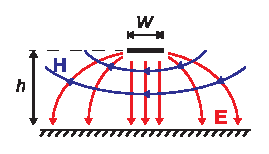
\includegraphics[width=2in]{modules/m0186_NarrowMicrostripEndView.eps} 
% https://commons.wikimedia.org/wiki/File:Electric_and_Magnetic_Fields_for_Microstrip.svg
}}{A microstrip of width capital W sits a distance small h above a plate. Electric field lines capital E point from the microstrip to the plate. The center lines have no curve and the lines emanating from each end bend down toward the plate. The magnetic field lines between the trace and the plate are approximately semicircular and point clockwise.}
\end{center}
\centerline{\scriptsize 
\copyright~\hyperref[m0186_fNarrow_Credit]{S.\ Lally}  
\href{https://creativecommons.org/licenses/by-sa/4.0/}{CC BY~SA 4.0} 
} 
\caption{
\label{m0186_fNarrow}
Electric and magnetic fields lines for narrow ($W \ll h$) microstrip line.
}
\end{figure}
%
\begin{figure} % <--- "[b!]" for first figure in section *only*; delete for 2nd and subsequent figures
\begin{center}
\pdftooltip{{  % note double braces
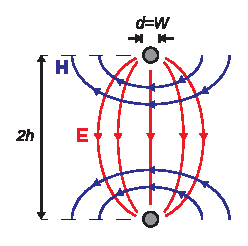
\includegraphics[width=2in]{modules/m0186_NarrowMicrostripEndViewTwinlineModel.eps} 
% https://commons.wikimedia.org/wiki ...
}}{Cross-section of 2 wires where upper wire is narrow microstrip with diameter equal to capital W. The wires are a distance 2 small h apart. The electric field lines, capital E, originate from the upper wire and terminate at the second wire. The magnetic field intensity, capital H, are concentric semi-circular loops. Upper loops point clockwise and lower loops point counter clockwise.
}
\end{center}
%\centerline{\scriptsize 
%\copyright~\hyperref[m0003_fBarMagnet_Credit]{Y.\ Qin} 
%\href{https://creativecommons.org/licenses/by/3.0/}{CC BY 3.0} 
%} % \centerline 
\caption{
\label{m0186_fNarrow2}
Noting the similarity of the fields in narrow microstrip line to those in a parallel wire line.
}
\end{figure}
%
\begin{figure} % <--- "[b!]" for first figure in section *only*; delete for 2nd and subsequent figures
\begin{center}
\pdftooltip{{  % note double braces
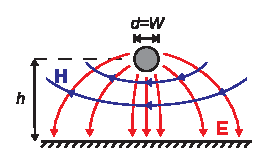
\includegraphics[width=2in]{modules/m0186_NarrowMicrostripEndViewTwinlineModel2.eps} 
% https://commons.wikimedia.org/wiki ...
}}{A microstrip above a plate. The microstrip has diameter small d equal to capital W.}
\end{center}
%\centerline{\scriptsize 
%\copyright~\hyperref[m0003_fBarMagnet_Credit]{Y.\ Qin} 
%\href{https://creativecommons.org/licenses/by/3.0/}{CC BY 3.0} 
%} % \centerline 
\caption{
\label{m0186_fNarrow3}
Modeling the fields in narrow microstrip line as those of a parallel wire line, now introducing the ground plane.
}
\end{figure}

Note that the field lines shown in Figure~\ref{m0186_fNarrow} are quite similar to those for parallel wire line (Section~\ref{m0188_Parallel_Wire_Transmission_Line}).
If we choose diameter $d=W$ and wire spacing $D=2h$,  
then the fields of the microstrip line in the dielectric spacer must be similar to those of the parallel wire line between the lines. 
This is shown in Figure~\ref{m0186_fNarrow2}.
Note that the fields above the dielectric spacer in the microstrip line will typically be somewhat different (since the material above the trace is typically different; e.g., air). 
However, it remains true that we expect most of the energy to be contained in the dielectric, so we shall assume that this difference has a relatively small effect.

Next, we continue to refine the model by introducing the ground plane, as shown in Figure~\ref{m0186_fNarrow3}: 
The fields in the upper half-space are not perturbed when we do this, since the fields in Figure~\ref{m0186_fNarrow2} already satisfy the boundary conditions imposed by the new ground plane.
Thus, we see that the parallel wire transmission line provides a pretty good guide to the structure of the fields for the narrow transmission line, at least in the dielectric region of the upper half-space.

We are now ready to estimate the characteristic impedance $Z_0\approx\sqrt{L'/C'}$ of low-loss narrow microstrip line.  
Neglecting the differences noted above, we estimate that this is roughly equal to the characteristic impedance of the analogous ($d=W$ and $D=2h$) parallel wire line. Under this assumption, we obtain from Equation~\ref{m0188_eZ0PWL}: 
 %
\begin{equation}
\boxed{
Z_0 \sim \frac{1}{\pi}\frac{\eta_0}{\sqrt{\epsilon_r}}\ln\left( 4h/W \right) ~~~ (W \ll h) 
\label{m0186_eZ0narrow}
}
\end{equation}
%
This estimate will exhibit only ``order of magnitude'' accuracy (hence the ``$\sim$'' symbol), since the contribution from the fields in half of the relevant space is ignored.  However we expect that Equation~\ref{m0186_eZ0narrow} will accurately capture the dependence of $Z_0$ on the parameters $\epsilon_r$ and $h/W$. These properties can be useful for making fine adjustments to a microstrip design.
%
%%%%%%%%%%%%%%%%%%%%%%%%%%%%%%%%%%%%%%%%%%%%%%%
%ORB HIGHLIGHT
\begin{mdframed}[backgroundcolor=yellow!20,nobreak=true] 
The characteristic impedance of ``narrow'' ($W \ll h$) microstrip line can be roughly approximated by Equation~\ref{m0186_eZ0narrow}.   
\end{mdframed}
%%%%%%%%%%%%%%%%%%%%%%%%%%%%%%%%%%%%%%%%%%%%%%%

{\bf Intermediate case.}   
An expression for $Z_0$ in the intermediate case -- even a rough estimate -- is difficult to derive, and beyond the scope of this book.
However, we are not completely in the dark, since we can reasonably anticipate that $Z_0$ in the intermediate case should be intermediate to estimates provided by the wide and narrow cases.
This is best demonstrated by example.
Figure~\ref{m0186_fFR4} shows estimates of $Z_0$ using the wide and narrow expressions (blue and green curves, respectively) for a particular implementation of microstrip line (see Example~\ref{m0186_exFR4} for details).
%
\begin{figure} % <--- "[b!]" for first figure in section *only*; delete for 2nd and subsequent figures
\begin{center}
\pdftooltip{{  % note double braces
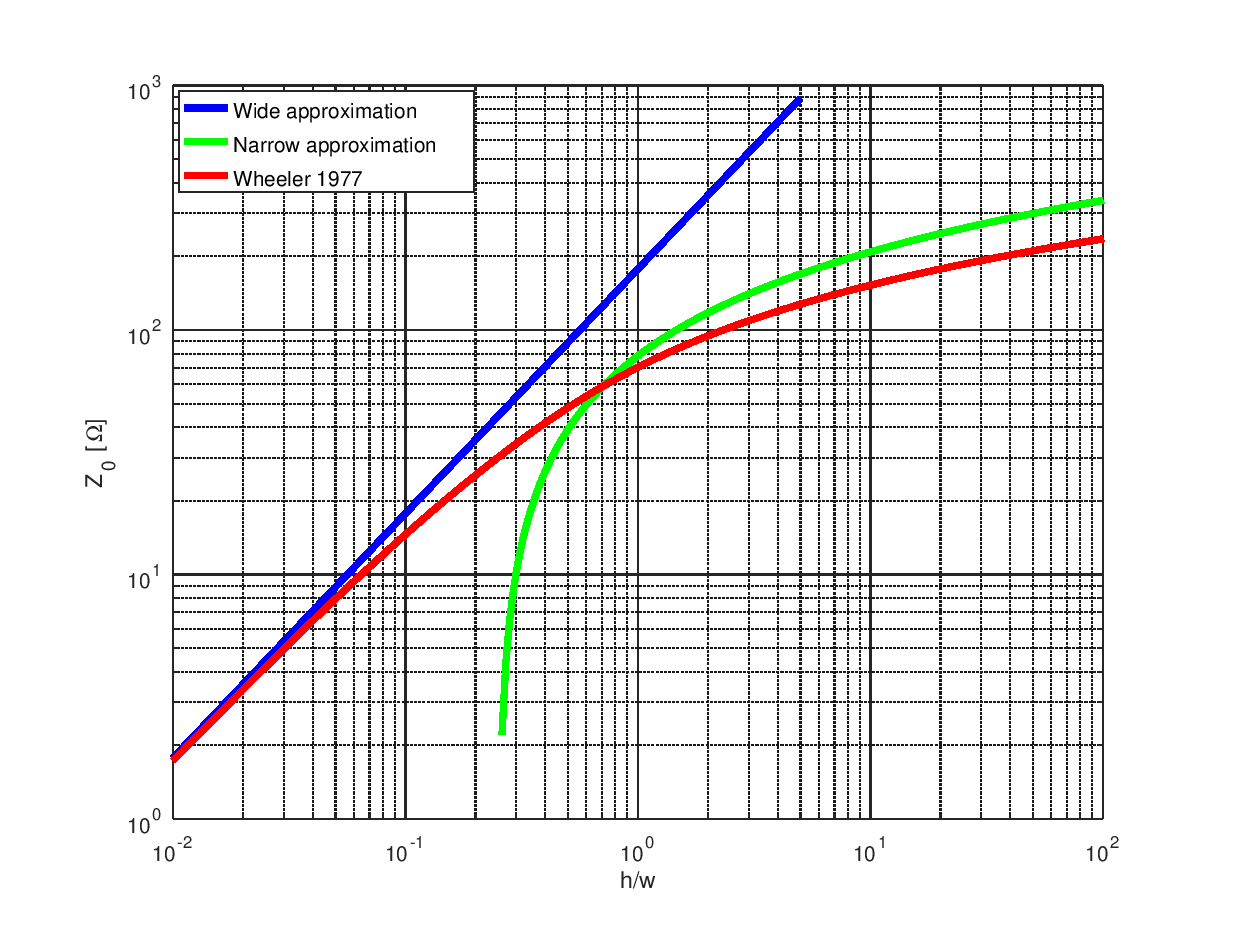
\includegraphics[width=\columnwidth]{modules/m0186_fFR4.eps} 
% https://commons.wikimedia.org/wiki/File:M0003_fBarMagnet.svg
}}{A log-log plot for small h divided by capital W versus capital Z subscript zero. Three lines plotted, wide approximation, narrow approximation, wheeler 1977 formula.}
\end{center}
%\centerline{\scriptsize 
%\copyright~\hyperref[m0003_fBarMagnet_Credit]{Y.\ Qin} 
%\href{https://creativecommons.org/licenses/by/3.0/}{CC BY 3.0} 
%} % \centerline 
\caption{
\label{m0186_fFR4}
$Z_0$ for FR4 as a function of $h/W$, as determined by the ``wide'' and ``narrow'' approximations, along with the Wheeler 1977 formula.  Note that the vertical and horizontal axes of this plot are in log scale.
}
\end{figure}
%
Since $Z_0$ varies smoothly with $h/W$, it is reasonable to expect that simply averaging the values generated using the wide and narrow assumptions would give a pretty good estimate when $h/W\sim 1$. 

However, it is also possible to obtain an accurate estimate directly.
A widely-accepted and broadly-applicable formula is provided in Wheeler 1977 (cited in ``Additional Reading'' at the end of this section).
This expression is valid over the full range of $h/W$, not merely the intermediate case of $h/W\sim 1$.
Here it is:
%
\begin{equation}
\begin{split}
Z_0 & \approx \frac{42.4~\Omega}{\sqrt{\epsilon_r+1}} ~\times \\
    &
\ln\left[
    1 +
    \frac{4h}{W'}
    \left( K + \sqrt{ K^2 + \frac{1+1/\epsilon_r}{2}\pi^2 } \right)
   \right]
\end{split}
\label{m0186_eWheeler10}
\end{equation}
% 
where
%
\begin{equation}
K \triangleq \frac{ 14 + 8/\epsilon_r }{ 11 } \left( \frac{4h}{W'} \right)
\end{equation}
%
and $W'$ is $W$ adjusted to account for the thickness $t$ of the microstrip line.  Typically $t\ll W$ and $t \ll h$, for which $W'\approx W$.
Although complicated, this formula should not be completely surprising.
For example, note the parameters $h$ and $W$ appear in this formula as the factor $4h/W$, which we encountered in the ``narrow'' approximation.
Also, we see that the formula indicates $Z_0$ increases with increasing $h/W$ and decreasing $\epsilon_r$, as we determined in both the ``narrow'' and ``wide'' cases.

The following example provides a demonstration for the very common case of microstrip implementation in FR4 
\index{FR4}
circuit board material.

%%%%%%%%%%%%%%%%%%%%%%%%%%%%%%%%%%%%%%%%%%%%%%%
%ORB EXAMPLE
~\\ \begin{example} 
\label{m0186_exFR4}
\begin{mdframed}[backgroundcolor=brown!20,linecolor=brown!20]\raggedright
Characteristic impedance of microstrip lines in FR4.
\\~\\
FR4 printed circuit boards consist of a substrate having $h\cong 1.575$~mm and $\epsilon_r\approx 4.5$.
Figure~\ref{m0186_fFR4} shows $Z_0$ as a function of $h/W$, as determined by the wide and narrow approximations, along with the value obtained using the Wheeler 1977 formula.
The left side of the plot represents the wide condition, whereas the right side of this plot represents the narrow condition.
The Wheeler 1977 formula is an accurate estimate over the entire horizontal span.
Note that the wide approximation is accurate only for $h/W<0.1$ or so, improving with decreasing $h/W$ as expected.
The narrow approximation overestimates $Z_0$ by a factor of about 1.4 (i.e., about 40\%). 
This is consistent with our previous observation that this approximation should yield only about ``order of magnitude'' accuracy. 
Nevertheless, the narrow approximation exhibits approximately the same rate of increase with $h/W$ as does the Wheeler 1977 formula.

Also worth noting from Figure~\ref{m0186_fFR4} is the important and commonly-used result that $Z_0\approx 50~\Omega$ is obtained for $h/W\approx 0.5$.
Thus, a $50~\Omega$ microstrip line in FR4 has a trace width of about 3~mm.   
\end{mdframed}
% note figures will need to go between "\end{mdframed}" and "\end{example}"
\end{example}
%%%%%%%%%%%%%%%%%%%%%%%%%%%%%%%%%%%%%%%%%%%%%%%

A useful ``take away'' from this example is that the wide and narrow approximations serve as useful guides for understanding how $Z_0$ changes as a function of $h/W$ and $\epsilon_r$.  This is useful especially for making adjustments to a microstrip line design once an accurate value of $Z_0$ is obtained from some other method; e.g., using the Wheeler 1977 formula or from measurements.

FR4 circuit board construction is so common that the result from the previous example deserves to be highlighted:
%
%%%%%%%%%%%%%%%%%%%%%%%%%%%%%%%%%%%%%%%%%%%%%%%
%ORB HIGHLIGHT
\begin{mdframed}[backgroundcolor=yellow!20,nobreak=true] 
In FR4 printed circuit board construction (substrate thickness $1.575$~mm, relative permittivity $\approx 4.5$, negligible trace thickness), $Z_0\approx 50~\Omega$ requires a trace width of about 3~mm.  $Z_0$ scales roughly in proportion to $h/W$ around this value.
\end{mdframed}
%%%%%%%%%%%%%%%%%%%%%%%%%%%%%%%%%%%%%%%%%%%%%%%

Simpler approximations for $Z_0$ are also commonly employed in the design and analysis of microstrip lines. 
These expressions are limited in the range of $h/W$ for which they are valid, and can usually be shown to be special cases or approximations of Equation~\ref{m0186_eWheeler10}.
Nevertheless, they are sometimes useful for quick ``back of the envelope'' calculations.

{\bf Wavelength in microstrip line.}
An accurate general formula for wavelength $\lambda$ in microstrip line is similarly difficult to derive.
A useful approximate technique employs a result from the theory of uniform plane waves in unbounded media.
For such waves, the phase propagation constant $\beta$ is given by
%
\begin{equation}
\beta = \omega\sqrt{\mu\epsilon}
\end{equation}
%
It turns out that the electromagnetic field structure for the guided wave in a microstrip line is similar in the sense that it exhibits TEM field structure, as does the uniform plane wave.
However, the guided wave is different in that it exists in both the dielectric spacer and the air above the spacer.  
Thus, we presume that $\beta$ for the guided wave can be approximated as that of a uniform plane wave in unbounded media having the same permeability $\mu_0$ but a different relative permittivity, which we shall assign the symbol $\epsilon_{r,eff}$ (for ``\emph{effective} relative permittivity''). 
\index{permittivity!effective}
Then:
%
\begin{flalign}
\beta &\approx \omega\sqrt{\mu_0~\epsilon_{r,eff}~\epsilon_0} ~~~\mbox{(low-loss microstrip)} \nonumber \\
      &=\beta_0 \sqrt{\epsilon_{r,eff}}
\end{flalign}
%
In other words, the phase propagation constant in a microstrip line can be approximated as the free-space phase propagation $\beta_0\triangleq\omega\sqrt{\mu_0\epsilon_0}$ times a correction factor $\sqrt{\epsilon_{r,eff}}$. 

Next, $\epsilon_{r,eff}$ is crudely approximated as the average of the relative permittivity of the dielectric slab and the relative permittivity of free space; i.e.,:
%
\begin{equation}
\epsilon_{r,eff} \approx \frac{\epsilon_r+1}{2}
\label{m0186_eeff}
\end{equation}
%  
Various refinements exist to improve on this approximation; however, in practice, variations in the value of $\epsilon_r$ for the dielectric due to manufacturing processes typically make a more precise estimate irrelevant.

Using this concept, we obtain
%
\begin{equation}
\lambda = \frac{2\pi}{\beta} = \frac{2\pi}{\beta_0\sqrt{\epsilon_{r,eff}}} = \frac{\lambda_0}{\sqrt{\epsilon_{r,eff}}}
\end{equation}
%
where $\lambda_0$ is the free-space wavelength
\index{wavelength!in microstrip}
$c/f$.
Similarly the phase velocity 
\index{phase velocity!in microstrip}
$v_p$ can be estimated using the relationship
%
\begin{equation}
v_p = \frac{\omega}{\beta} = \frac{c}{\sqrt{\epsilon_{r,eff}}}
\end{equation}
%
i.e., the phase velocity in microstrip is slower than $c$ by a factor of $\sqrt{\epsilon_{r,eff}}$.

%ORB EXAMPLE
~\\ \begin{example} 
\begin{mdframed}[backgroundcolor=brown!20,linecolor=brown!20]\raggedright
Wavelength and phase velocity in microstrip in FR4 
\index{FR4}
printed circuit boards.
\index{printed circuit board (PCB)}
\\~\\
FR4 is a low-loss fiberglass epoxy dielectric that is commonly used to make printed circuit boards (see ``Additional Reading'' at the end of this section).
For FR4, $\epsilon_r\approx 4.5$. 
The effective relative permittivity is therefore:
%
\begin{equation}
\epsilon_{r,eff}\approx(4.5+1)/2 = 2.75
\nonumber
\end{equation}
%
Thus, we estimate the phase velocity for the wave guided by this line to be about $c/\sqrt{2.75}$; i.e., 60\% of $c$.
Similarly, the wavelength of this wave is about 60\% of the free space wavelength.
In practice, these values are found to be slightly less; typically 50\%--55\%.
The difference is attributable to the crude approximation of Equation~\ref{m0186_eeff}.
\end{mdframed}\end{example}

%------------------------------------

{\bf Additional Reading:}
\begin{itemize}
\item ``\href{https://en.wikipedia.org/wiki/Microstrip}{Microstrip}'' on Wikipedia.
\item ``\href{https://en.wikipedia.org/wiki/Printed_circuit_board}{Printed circuit board}'' on Wikipedia.
\item ``\href{https://en.wikipedia.org/wiki/Stripline}{Stripline}'' on Wikipedia.
\item ``\href{https://en.wikipedia.org/wiki/Single-ended_signaling}{Single-ended signaling}'' on Wikipedia.
\item Sec.~8.7 (``Differential Circuits'') in S.W.~Ellingson, \emph{Radio Systems Engineering}, Cambridge Univ.\ Press, 2016. 
\item H.A.\ Wheeler, ``Transmission Line Properties of a Strip on a Dielectric Sheet on a Plane,'' {\it IEEE Trans.\ Microwave Theory \& Techniques}, Vol.~25, No.~8, Aug~1977, pp.~631--47. % http://dx.doi.org/10.1109/TMTT.1977.1129179.
\item ``\href{https://en.wikipedia.org/wiki/FR-4}{FR-4}'' on Wikipedia.
\end{itemize}
 
\index{microstrip|)}

